\textit{TicTacker} hace uso de diferentes clases que se comunican entre sí y que utilizan los elementos XML de Android para gestionar la vista correspondiente. Adicionalmente, se hace uso de una base de datos SQLite para gestionar los usuarios, los fichajes y las configuraciones personalizadas.

\subsection{Clases}
La aplicación cuenta con diferentes clases Java diferenciadas que dan respuesta a una o varias de las funcionalidades de la aplicación. A continuación se describen las siguientes clases utilizadas, pudiendo ver las relaciones entre las mismas por medio de diagrama de clases de la Figura \ref{fig:diagrama}.

\subsubsection{Activities}
\begin{itemize}
  \item \textbf{MainActivity}: actividad principal que se encarga de gestionar la navegación y la interfaz de usuario principal de la aplicación.
  \item \textbf{LoginActivity}: gestiona la autentificación de usuarios existentes, validando credenciales y guardando la sesión.
  \item \textbf{SignupActivity}: gestiona el registro de nuevos usuarios, incluyendo validación de los datos, que no se repitan usuarios y creación de cuentas.
  \item \textbf{SettingsActivity}: ofrece opciones de personalización de la aplicación, como cambiar el idioma o la jornada laboral.
\end{itemize}

\subsubsection{Fragments}
\begin{itemize}
  \item \textbf{ClockInFragment}: fragment que permite a los usuarios registrar sus fichajes, mostrando el estado actual y el tiempo trabajado.
  \item \textbf{HistoryFragment}: fragment que muestra el historial de fichajes del usuario, permitiendo exportar e importar datos por medio de ficheros CSV.
  \item \textbf{SettingsFragment}: fragment que permite a los usuarios ajustar sus preferencias, como las horas de trabajo semanales y los días laborables.
\end{itemize}

\subsubsection{Adaptadores}
\begin{itemize}
  \item \textbf{FichajeAdapter}: utilizado para mostrar listas de fichajes a través de un \textit{RecyclerView}.
\end{itemize}

\subsubsection{Clases generales}
\begin{itemize}
  \item \textbf{TicTacker}: clase principal de la aplicación que se encarga de aplicar las preferencias de usuario al iniciar.
  \item \textbf{Fichaje}: entidad que representa un fichaje con los atributos correspondiente, usado para instanciar objetos fácilmente con su fecha, hora de entrada, hora de salida, latitud, longitud y nombre de usuario para almacenar en la base de datos.
  \item \textbf{WorkTimeCalculator}: clase que proporciona métodos para calcular el tiempo trabajado y el tiempo restante.
\end{itemize}

\subsubsection{Helpers}
\begin{itemize}
  \item \textbf{DatabaseHelper}: gestiona la base de datos SQLite, incluyendo la creación de tablas y las operaciones.
  \item \textbf{NotificationHelper}: clase que gestiona la creación y envío de notificaciones.
\end{itemize}

\subsubsection{Eventos}
\begin{itemize}
  \item \textbf{FichajeEvents}: clase que gestiona los eventos relacionados con los fichajes, permitiendo notificar cambios a los listeners registrados.
\end{itemize}

\subsubsection{Workers}
\begin{itemize}
  \item \textbf{WorkTimeCheckWorker}: worker que comprueba periódicamente el tiempo trabajado y envía notificaciones al usuario si alcanza su jornada laboral.
\end{itemize}

\subsection{Diagrama de clases}

\begin{figure}[H]
    \centering
    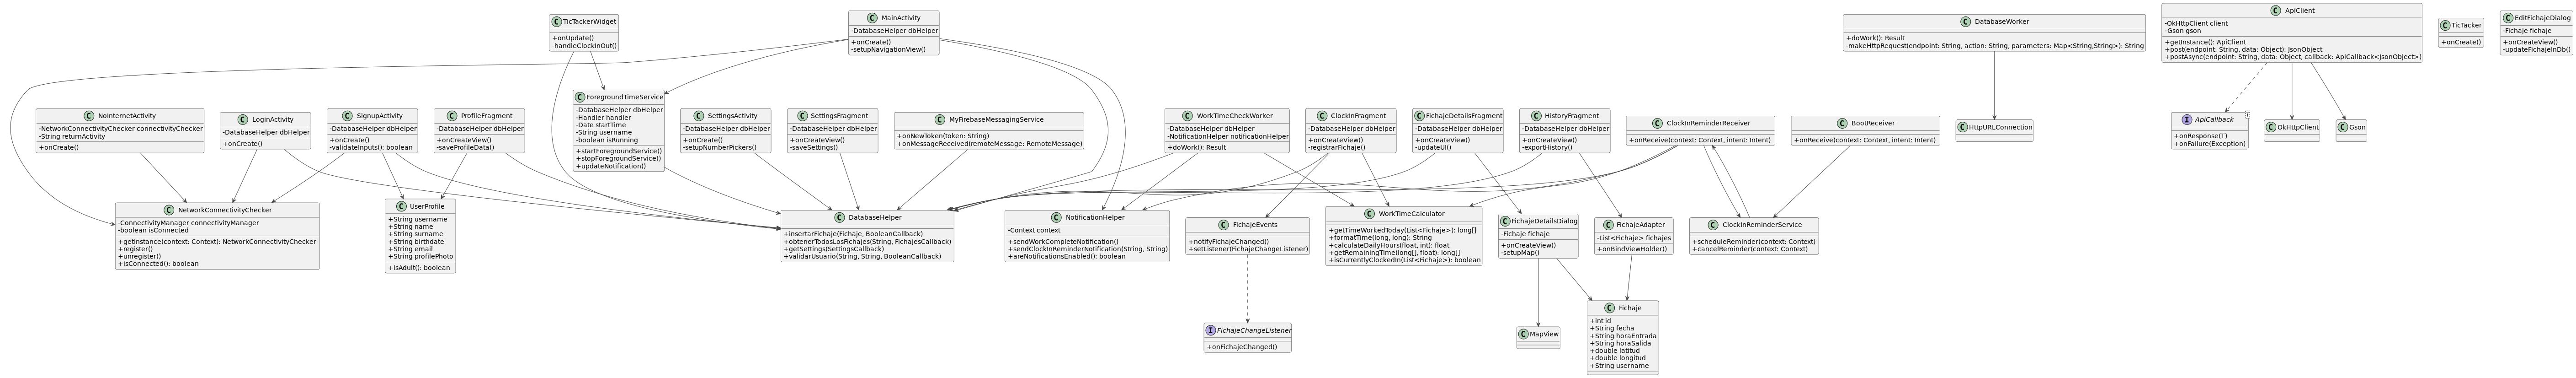
\includegraphics[width=1\linewidth]{root/diagrama.png}
    \caption{Diagrama de clases del proyecto}
    \label{fig:diagrama}
\end{figure}

\subsection{Base de datos}

Además de las \textit{SharedPreferences}, para gestionar la persistencia de la aplicación se hace uso de una base de datos de tipo SQLite. La base de datos está definida por la clase \textit{DatabaseHelper}, que extiende de \textit{SQLiteOpenHelper}, y contiene las siguientes tablas:

\begin{itemize}
  \item \textbf{Tabla Fichajes}: almacena la información sobre los fichajes de los usuarios.
  \begin{itemize}
    \item \textbf{Atributos principales}: \texttt{id}, \texttt{fecha}, \texttt{hora\_entrada}, \texttt{hora\_salida}, \texttt{latitud}, \texttt{longitud}, \texttt{username}.
    \item \textbf{Índices}: \texttt{id} es un campo único y clave primaria.
  \end{itemize}
  \item \textbf{Tabla Configuraciones}: almacena las configuraciones de horas de trabajo y días laborables.
  \begin{itemize}
    \item \textbf{Atributos principales}: \texttt{id}, \texttt{weekly\_hours}, \texttt{working\_days}.
    \item \textbf{Índices}: \texttt{id} es un campo único y clave primaria.
  \end{itemize}
  \item \textbf{Tabla Usuarios}: almacena los usuarios registrados en la aplicación.
  \begin{itemize}
    \item \textbf{Atributos principales}: \texttt{id}, \texttt{username}, \texttt{password}.
    \item \textbf{Índices}: \texttt{username} es un campo único indexado para prevenir duplicados.
  \end{itemize}
\end{itemize}
